
\begin{flushleft}

	\bigskip
	\begin{figure}[h!]
		\centering
		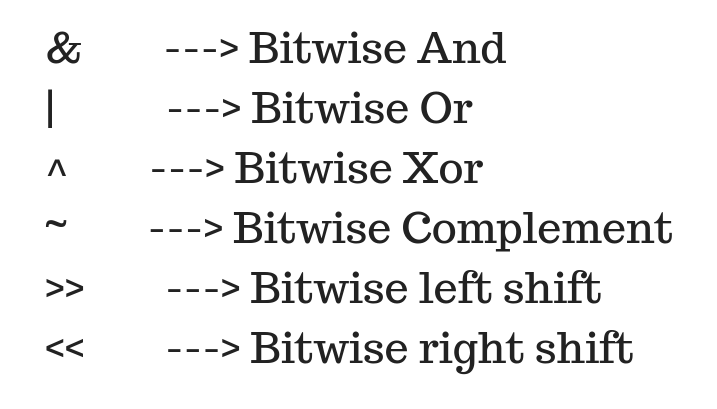
\includegraphics[scale=0.5]{content/chapter3/images/bitwise2.png}
	\end{figure}
	
	\begin{tabular}{|p{10em}|p{8em}|p{6em}|}
		
		\multicolumn{3}{l}{} \\
		\multicolumn{3}{l}{\textbf{Bitwise \&} - If both bits are 1, then only 1 otherwise 0}                  
		\\ \hline
		\multicolumn{1}{|l|}{Sample Code} & \multicolumn{1}{l|}{Output}  & \multicolumn{1}{l|}{Explaination}   
		\\ \hline
		\multicolumn{1}{|l|}{\begin{tabular}[c]{@{}l@{}}int a=4; \\
				int b=5; \\
				System.out.println(a \& b)	 \end{tabular}}  & 
		\multicolumn{1}{l|}{4}   &  
		\multicolumn{1}{|l|}{\begin{tabular}[c]{@{}l@{}}100 \\
				101 \\
				----- \\
				100	 \end{tabular}}  
		\\ 
		\hline
	
		\multicolumn{3}{l}{} \\
		\multicolumn{3}{l}{\textbf{Bitwise |} - If atleast one bit is 1, then only 1 otherwise 0}                  
		\\ \hline
		\multicolumn{1}{|l|}{Sample Code} & \multicolumn{1}{l|}{Output}  & \multicolumn{1}{l|}{Explaination}   
		\\ \hline
		\multicolumn{1}{|l|}{\begin{tabular}[c]{@{}l@{}}int a=4; \\
				int b=5; \\
				System.out.println(a | b)	 \end{tabular}}  & 
		\multicolumn{1}{l|}{5}   &  
		\multicolumn{1}{|l|}{\begin{tabular}[c]{@{}l@{}}100 \\
				101 \\
				----- \\
				101	 \end{tabular}}  
		\\ 
		\hline
	
		
	\end{tabular}
	
	\newpage
	
	\begin{tabular}{|p{10em}|p{8em}|p{8em}|}
		
		\multicolumn{3}{l}{} \\
		\multicolumn{3}{l}{\textbf{Bitwise \^} - Also called x-or. If both bits are different, then 1, otherwise 0}                  
		\\ \hline
		\multicolumn{1}{|l|}{Sample Code} & \multicolumn{1}{l|}{Output}  & \multicolumn{1}{l|}{Explaination}   
		\\ \hline
		\multicolumn{1}{|l|}{\begin{tabular}[c]{@{}l@{}}int a=4; \\
				int b=5; \\
				System.out.println(a \textbf{\^} b)	 \end{tabular}}  & 
		\multicolumn{1}{l|}{1}   &  
		\multicolumn{1}{|l|}{\begin{tabular}[c]{@{}l@{}}100 \\
				101 \\
				----- \\
				001	 \end{tabular}}  
		\\ 
		\hline
		
		\multicolumn{3}{l}{} \\
		\multicolumn{3}{l}{\textbf{Bitwise \~} - Bitwise complement operator, 1 becomes 0 and 0
becomes 1}                  
		\\ \hline
		\multicolumn{1}{|l|}{Sample Code} & \multicolumn{1}{l|}{Output}  & \multicolumn{1}{l|}{Explaination}   
		\\ \hline
		\multicolumn{1}{|l|}{\begin{tabular}[c]{@{}l@{}}int a=4; \\
				System.out.println( \textbf{\~} a)	 \end{tabular}}  & 
		\multicolumn{1}{l|}{-5}   &  
		\multicolumn{1}{|l|}{\begin{tabular}[c]{@{}l@{}} 32-bit os represents number with	\\
				total 32 bits as 000...000100 \\
				 \textbf{\~} 000...000100 = 111...111011 \\
				Left most bit is sign bit where, \\
				1 is negative and 0 is positive \\
				Since left most bit is now 1, number is negative \\
				Negative number is represented as \\
				1's complement + 1 \\
				ie. 100..000100 + 1 = 100...000101	
		 \end{tabular}}  
		\\ 
		\hline
	

		\multicolumn{3}{l}{} \\
		\multicolumn{3}{l}{\begin{tabular}[c]{@{}l@{}}\textbf{Bitwise >>} - Bitwise right shift. \\
		Remove "x" bit from right side and add "x" 0 to left side.	 \end{tabular}}                  
		\\ \hline
		\multicolumn{1}{|l|}{Sample Code} & \multicolumn{1}{l|}{Output}  & \multicolumn{1}{l|}{Explaination}   
		\\ \hline
		\multicolumn{1}{|l|}{\begin{tabular}[c]{@{}l@{}}int a=10; \\
				int x=2; \\
				System.out.println(a >> x)	 \end{tabular}}  & 
		\multicolumn{1}{l|}{2}   &  
		\multicolumn{1}{|l|}{\begin{tabular}[c]{@{}l@{}}000...1010 >> 2 \\
				000...0010 \\
					 \end{tabular}}  
		\\ 
		\hline
	\end{tabular}

	\newpage
	
	\begin{tabular}{|p{10em}|p{8em}|p{6em}|}
		
		
	\multicolumn{3}{l}{} \\
	\multicolumn{3}{l}{\begin{tabular}[c]{@{}l@{}}\textbf{Bitwise <<} - Bitwise left shift. \\	
	Remove "x" bit from left side and add "x" 0 to right side.	 \end{tabular}}                  
	\\ \hline
	\multicolumn{1}{|l|}{Sample Code} & \multicolumn{1}{l|}{Output}  & \multicolumn{1}{l|}{Explaination}   
	\\ \hline
	\multicolumn{1}{|l|}{\begin{tabular}[c]{@{}l@{}}int a=10; \\
			int x=2; \\
			System.out.println(a << x)	 \end{tabular}}  & 
	\multicolumn{1}{l|}{40}   &  
	\multicolumn{1}{|l|}{\begin{tabular}[c]{@{}l@{}}000...1010 << 2 \\
			000...101000 \\
	\end{tabular}}  
	\\ 
	\hline
		
	\end{tabular}
		
	\noteblock{
		\begin{itemize}
			\item \&, | , \textbf{\^}  are applicable for both boolean and integral type.
			\item >> , << are applicable for integral type only.
			\item \textbf{\~} applicable for only integral type but not for boolean type.
		\end{itemize}	
	}
		
		
\end{flushleft}
